\subsection{Distanz}

Die Distanzkalkulation zwischen zwei Punkten ist in der selben, oben beschriebenen, Webapp implementiert. Hierzu gibt es zwei Eingabefelder, in die Koordinaten in einem beliebigen der oben genannten Formate eingegeben oder einkopiert werden können. Die Koordinaten werden anschließend in Dezimalgrad umgerechnet. Mittel der Haversine Formel wird die Distanz zwischen den beiden Punkten ermittelt und ausgegeben.

Zusätzlich sind die Beispiele aus der Angabe mit der jeweiligen Distanz enthalten. Durch Klicken auf die Koordinaten können diese auch direkt in die interaktive Distanzermittlung übernommen werden. Außerdem ist natürlich ein Kopieren und Einfügen möglich.

\begin{figure}[h]
    \centering
    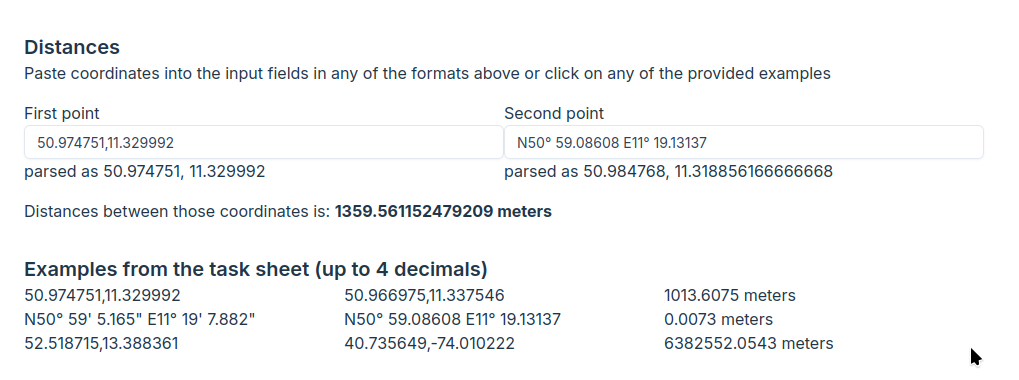
\includegraphics[width=0.9\textwidth]{figures/distanzkalkulation.png}
    \caption{Screenshot aus der WebApp. Zu sehen sind hier neben den Distanzen zu den Beispielen aus der Angabe auch die mögliche Mischung von Eingabeformaten.}
    \label{distanzkalkulation}
\end{figure}